`\section{Design Process} % Talk about the Design Process

%TODO: Add an introduction to the Design Process

    \subsection{Mechanical Design} 

        \subsubsection{Design Requirements}
            \begin{Deliverables}
                \item Lab-appropriate size
                \item Additive Manufacturing method with polyactic acid (PLA)
                \item Modular \& Adaptable to change
                \item High coefficient of friction with the ground
                \item Able to move leg both forward/backward and sideways
                \item Powerful and speedy motors that can sustain the weight of the robot
                \item Head and tail that can be used to shift center of mass of the robot
                \item Aesthetically pleasing
            \end{Deliverables}
            
         \subsubsection{Mechanical Design Process}
            The mechanical design of SmallKat was very important. The robot needed to be balanced and designed properly so that the motors would be able to move the whole system and be able to properly walk. It also needed to be designed in a way that was easy to modify or change out components if users wanted to change something or needed to fix a part that had broken. The mechanical design process can be broken down into several steps. 
             \begin{Deliverables}
                \item 3 DOF vs 4 DOF
                \item Motor Selection and Testing
                \item Kinematics and Analysis
                \item Tail Design and Iterations
                \item Design Iterations
            \end{Deliverables}
      
        \subsubsection{3-DoF vs 4-DoF}
            The leg design was the most important of decisions when designing SmallKat mechanically. The first decision was to decide how many degrees of freedom our system would have. More degrees would allow for more flexibility and give users more options for gait designs. However, too many degrees of freedom per leg would not only complicate control algorithms, but also increase weight per leg, which would in turn increase rotational and linear inertia, add more strain to the motors, and decrease dynamic gait performance. It is important to note that SmallKat needed at least 3 degrees of freedom to allow for forward and sideways movement, necessary for dynamic walking. Therefore, the decision was between 3 and 4 DoFs.

            Early on in our design process, we spoke to Boston Dynamics (as talked about in Section \ref{subsec:BostonDynamicsInterview}), and one of the questions we asked was their opinion on 3-DoF vs 4-DoF legs. In their research, they saw the design simplicity to be the major benefit of 3-DoF legs, so almost all of their quadrupeds were 3 degrees of freedom; a simpler design means less can go wrong for their customers. However, the engineers did admit they didn't look into different 4-DoF leg designs.

                \begin{figure}[H]
                    \centering
                    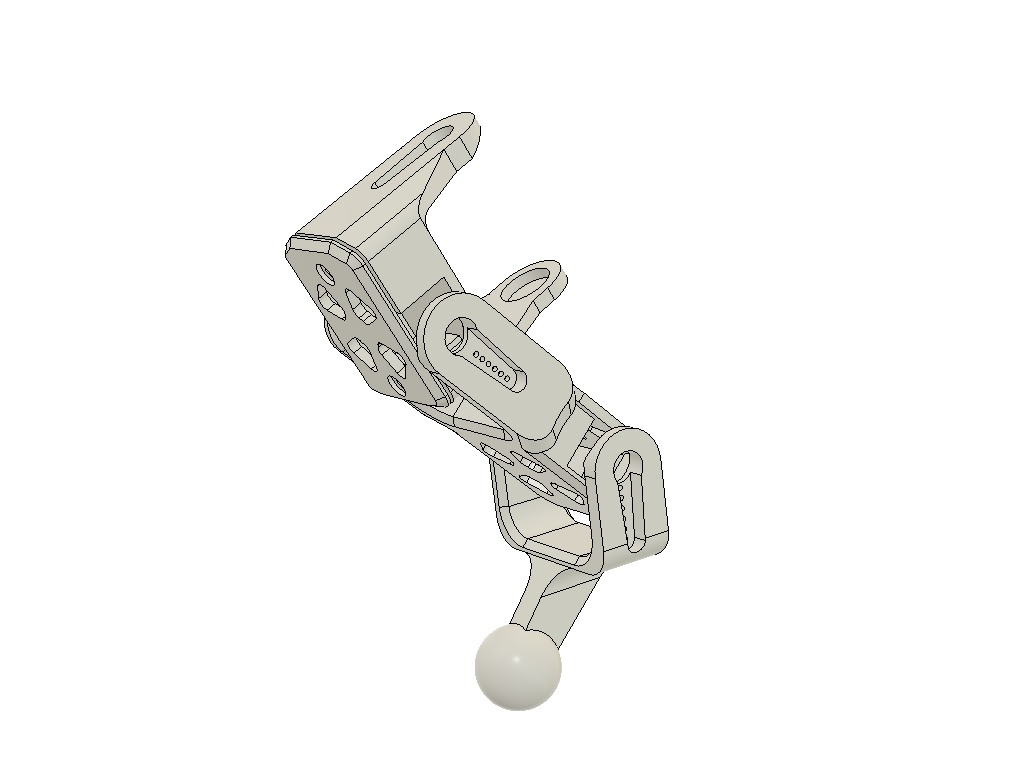
\includegraphics[width=0.7\textwidth]{figures/3dof.png}
                    \caption{Planar 3-DoF Leg Design}
                    \label{fig:3DoFDesign}
                \end{figure}
                
                \begin{figure}[H]
                    \centering
                    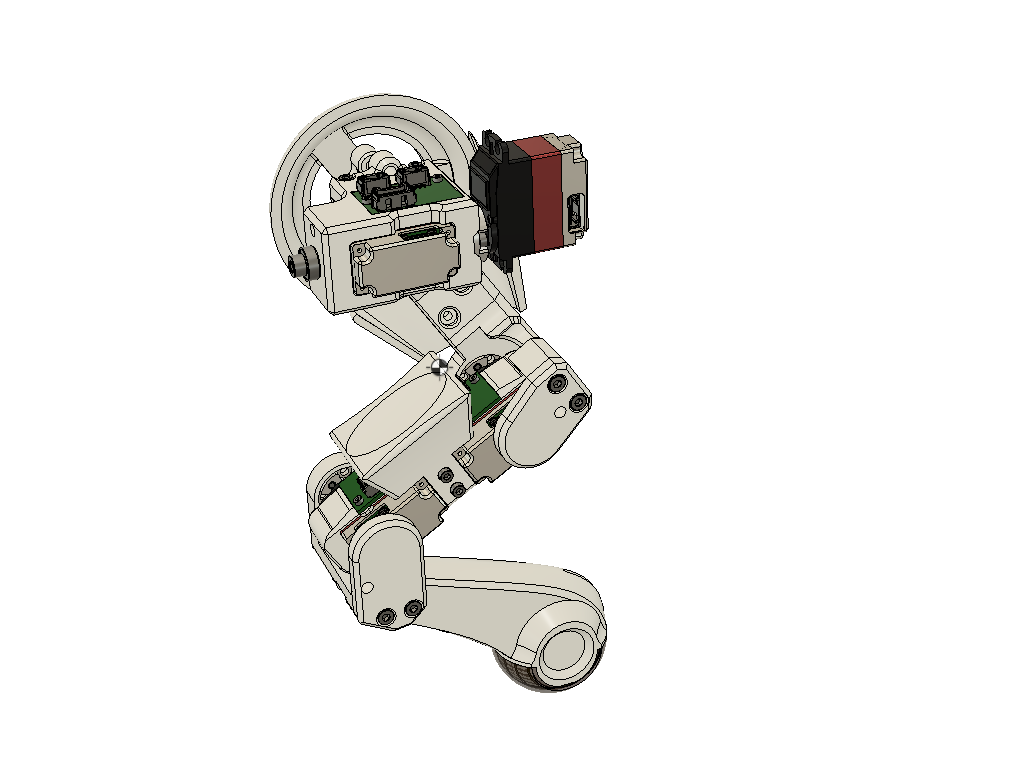
\includegraphics[width=0.7\textwidth]{figures/4dof.png}
                    \caption{Planar 4-DoF Leg Design}
                    \label{fig:4DoFDesign}
                \end{figure}
                
            After some deliberation and research, we ultimately decided to take a different approach to a 4-DoF leg: a 3-DoF planar manipulator with a rotation axis in the hip, as depicted in Figure \ref{fig:Planar4DoF}. This would give the platform the capability to change the angle of contact with the ground, potentially improving performance on irregular terrain. This novel leg design, we call a planar 4-DoF Leg, is different from any other quadruped we found in our research. Our initial concern of not having enough speed and power in the motors we selected were taken care of after some testing (see Section \ref{subsubsec:MotorSelection}). However, the main reason we chose 4-DoF legs instead of the 3-DoF variant was the adaptability it gave the users of our platform. Additionally because it has not been done before in any of the quadrupedal robot systems we have found it offered a unique opportunity to research the difference between 3 DOF and 4 DOF systems. 
            
        \subsubsection{Motor Selection and Testing}\label{subsubsec:MotorSelection}
        One of the most important parts of any robot is it's motors. We considered many different motor solutions for this project, including standard hobby servos, planetary geared motors, and "smart" motors from companies like Dynamixel and Maxon. Our decision - standard hobby servos - was mostly based on the selection and standard that has been formed in the hobby industry. If a user wanted to replace their motors with weaker or more powerful version, he or she could, assuming the servo they purchase are the same size as the ones we designed around. This gives the users the option of motors to use based on their needs and budget. 
            \paragraph{Motor Options}
            Based on the size, we found a few options of different motors we can use. These include a standard (modified) hobby servo (Jx-Servo HV-5932MG) and 2 Dynamixel motors. Table \ref{tab:MotorComparison} lists the pros and cons for each option we considered.

            \begin{table} [H]
                \centering
                    \begin{tabular}{|p{0.2\linewidth}|p{0.35\linewidth}|p{0.35\linewidth}|}
                        \hline
                        Motor & Pros & Cons \\
                        \hline
                        \multirow{4}{*}{HV-5932MG}& Low Cost  & No Feedback\\
                            & Available in high torque variants & Can only perform position control\\
                            & Simple mounting style & Unable to tune PID\\
                            & Easy Communication Style & Non daisy-chainable \\
                            \hline
                        \multirow{4}{*}{Dynamixel AX-12a}  & Mid range  Cost   &  Low Torque\\
                            & Easy to mount & Difficult Communication protocol \\
                            & Allows for daisy chaining & Large body\\
                            & Allows for tuned PID & \\
                            & Allows for Position, Velocity and torque control& \\
                            \hline
                        \multirow{4}{*}{Dynamixel XH430}  & High Torque  & Expensive\\
                            & Easy to mount & Difficult Communication protocol \\
                            & Allows for daisy chaining & Large body \\
                            & Allows for tuned PID & \\
                            & Allows for Position, Velocity and torque control& \\
                        \hline
                    \end{tabular}
                    \caption{Pros \& Cons for each motor considered}
                    \label{tab:MotorComparison}
                \end{table}
                
            \paragraph{Motor Decision}
                Ultimately we decided to use the Hobby Servo. While the Dynamixel servos provided an all in one solution to the sensor integration and feedback we were looking for in our motors, the price for the amount of power we needed was way out of our budget. As a result we needed to come up with an alternative solution for providing feedback to our system. While we could have just added external sensors to our motors and joints, we decided to modify the servos to suit our needs. This was also part of our decision to choose the hobby servos, because after some research and thinking we discovered that we could fit our own electronics board and housing on the servos to essentially turn them into the smart Dynamixel servos for a fraction of the cost. The design of the servo electronics board is covered in more depth in the electrical implementation section of this paper.
                
            \paragraph{Elastics Testing} 0o[h]

                Once we had decided on a servo we had a rough idea of the size of the robot we were intending to create. Based on this conceptual size and weight and the size and power of our servos,  we felt that there was a possibility that an elastic suspension system would be needed to allow the robot to function properly. This system would work by attaching a spring or bungee cord or other elastic mechanism to the joints of the cat. When the cat is under its own weight the elastics work to reduce the amount of torque seen by the motor. Because most elastic systems are dependent on the distance they are compressed or extended by the farther the limb is moved the more additional torque is applied. One thing to keep in mind is that when the robot has lifted up the leg and is no longer under its own weight the elastic systems are now working against the motor. This means that however much additional assistance is applied by the springs, it can not be greater than the max torque output of the motor.  In order to get an idea of the spring constants available we purchased a length of ¼ bungee cord to test. The test was done by suspending a length of bungee cord from the top of a table and hanging weights on it to determine how far it stretches.  Given that Hooke's law is F = k*x where k is the spring constant and x is a linear distance we can easily determine the value of the spring constant. 
	
	            \begin{figure}[H]
                    \centering
                    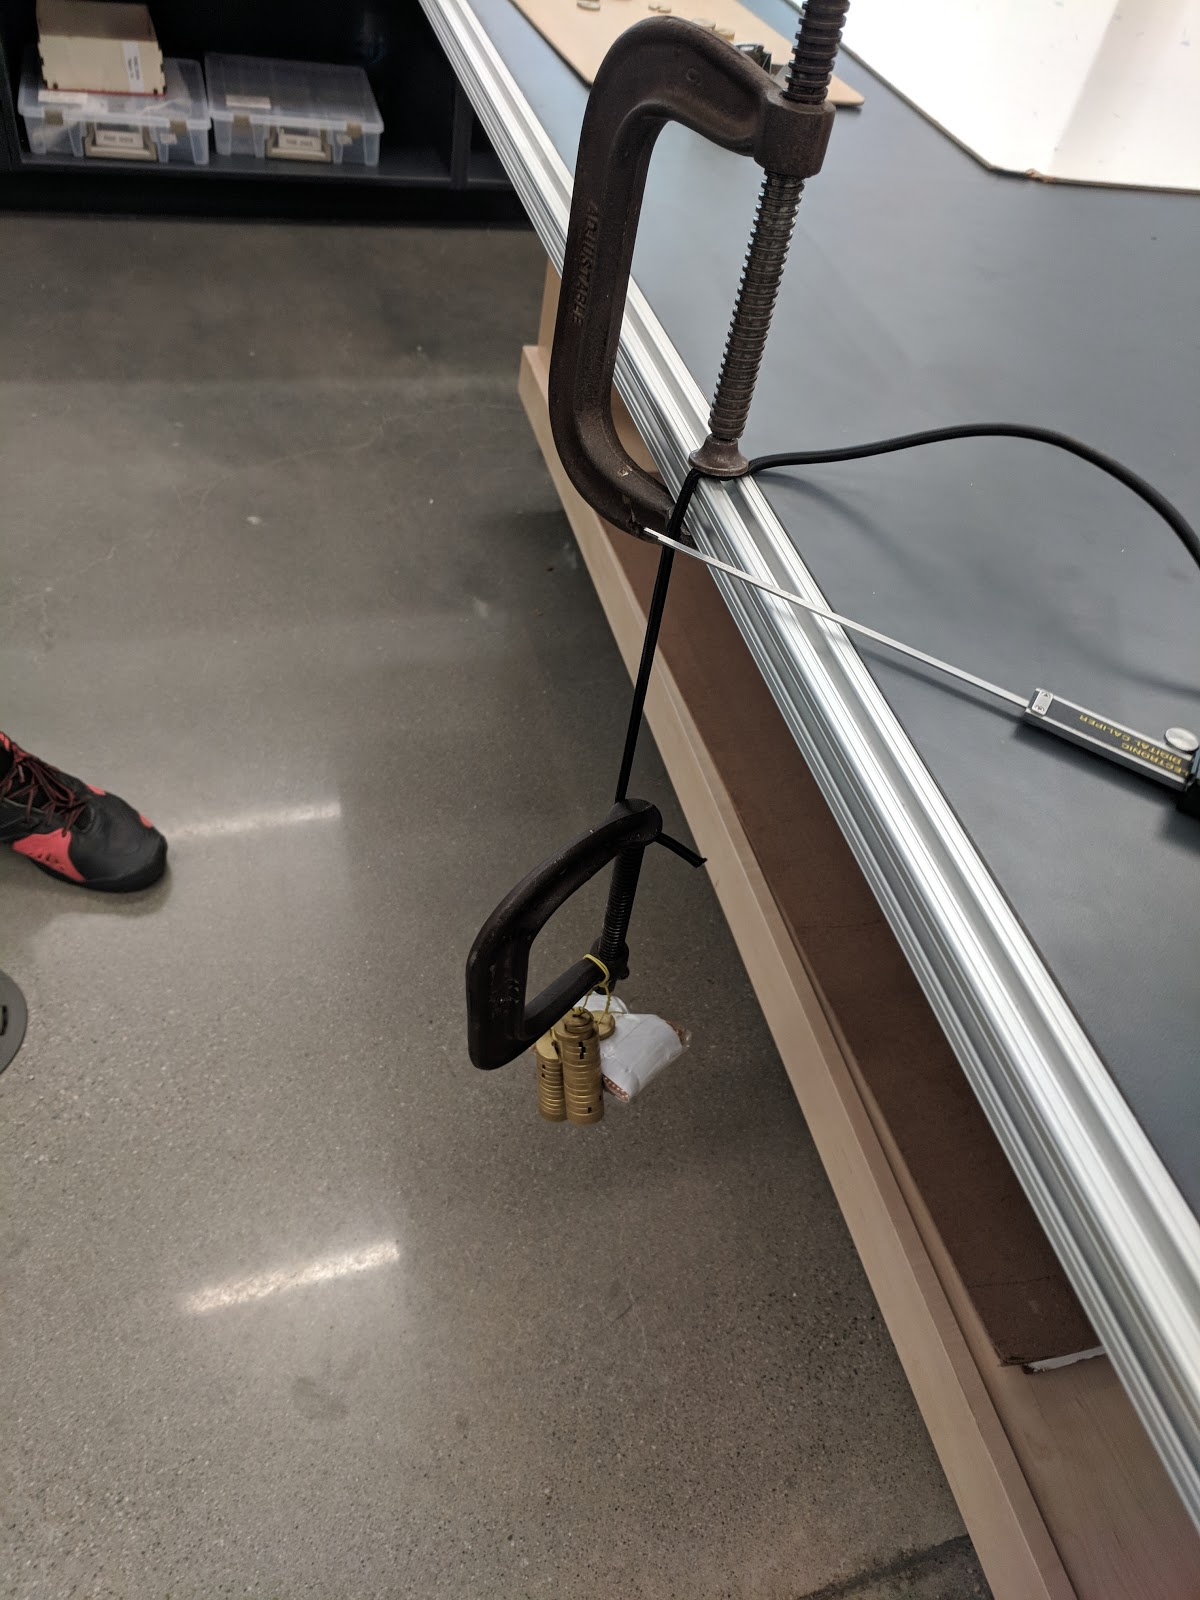
\includegraphics[width=0.7\textwidth]{figures/Spring testing.jpg}
                    \caption{Elastics Testing}
                    \label{fig:ElasticsTestingGraphic}
                \end{figure}
	
                \begin{table} [H]
                \centering
                    \begin{tabular}{|c|c|c|c|c|}
                        \hline
                        Test & Weight & Initial Distance & Final Distance & k\\
                        \hline
                        1 & 2 kg & 13.0 cm & 16.5 cm & .57 kg/cm \\
                        \hline
                        2 & 2.7 kg & 13.0 cm & 18.75 cm & .47 kg/cm \\
                        \hline
                    \end{tabular}
                    \caption{Spring Test:  Tested bungee cords to determine the spring constant value}
                    \label{tab:MotorComparison}
                \end{table}

                Our tests weren't perfect but they gave us a rough idea of what to expect for the spring constant of our elastics. Using this info we figured we could make a rough controller for the system and refine it once we had better tests using the motors. However, we actually ended up not using elastics because the results of the motor testing proved that the motors would be powerful enough to move the robot.
                
            
            \paragraph{Motor Testing} \label{par:MotorTesting}
                Once the servo was chosen, we tested the actual torque output of several motors. This was done to confirm the specifications given to us by the supplier as well as to see the difference between motors of the same model. Knowing the motors' limits is crucial when designing the quadruped. To test our servos we created a laser cut lever arm with holes spaced 1 cm apart. By hanging a 1kg weight on the holes with the lever parallel to the ground and moving incrementally outward we could determine the actual torque output of the motor. We tested both the stall torques and operational torques. The operational torque was determined by adding weight until the motor could no longer move the weight. The stall torque was determined by adding weight until the motor could not physically hold the weight up.

                \begin{figure}[H]
                    \centering
                    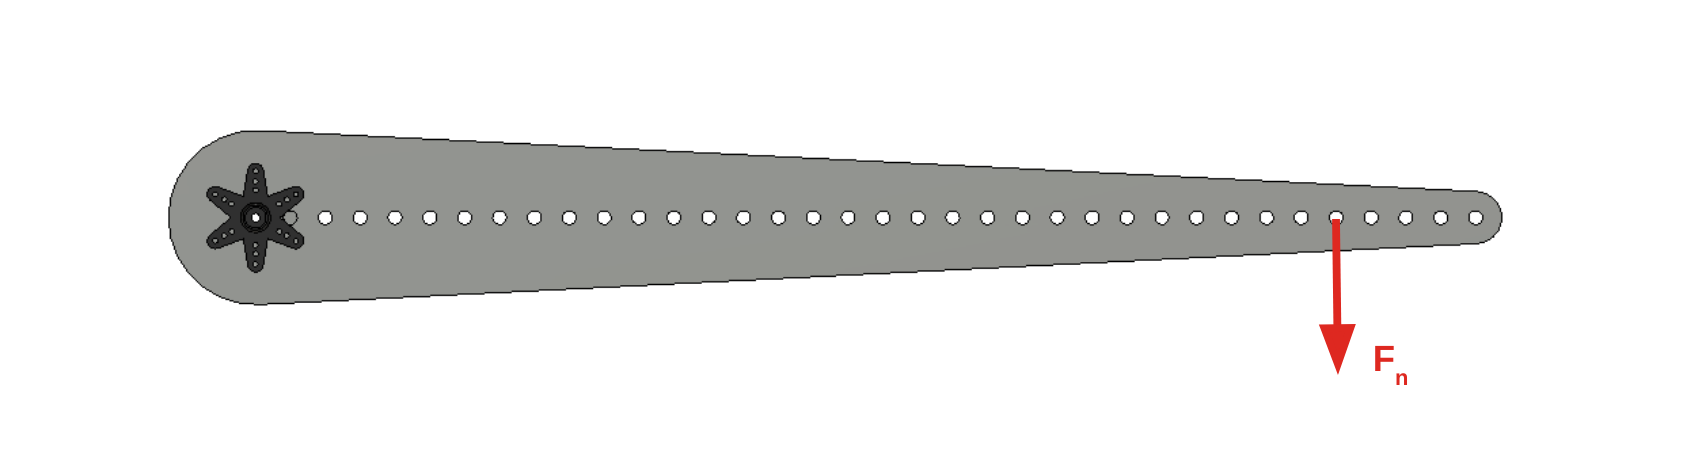
\includegraphics[width=0.7\textwidth]{figures/MotorTestingDiagram.png}
                    \caption{Graphic of how motors were tested}
                    \label{fig:MotorTestingGraphic}
                \end{figure}

                The HV-5932MG servos are advertised with a stall torques of 32 kg-cm. We found the servo was able to hold the 1kg weight at the 32 cm however it could not move it which is to be expected given that is its stall torque. From there we moved the weight closer in to determine at what point the servo could comfortably move the weight. We found that 20 kg-cm was the highest torque the servo could operate without any loss of function. Using this number as the known output torque of the motor will allow us to design a system that we are confident will be able to operate without falling down under its own weight.


                \begin{figure}[H]
                    \centering
                    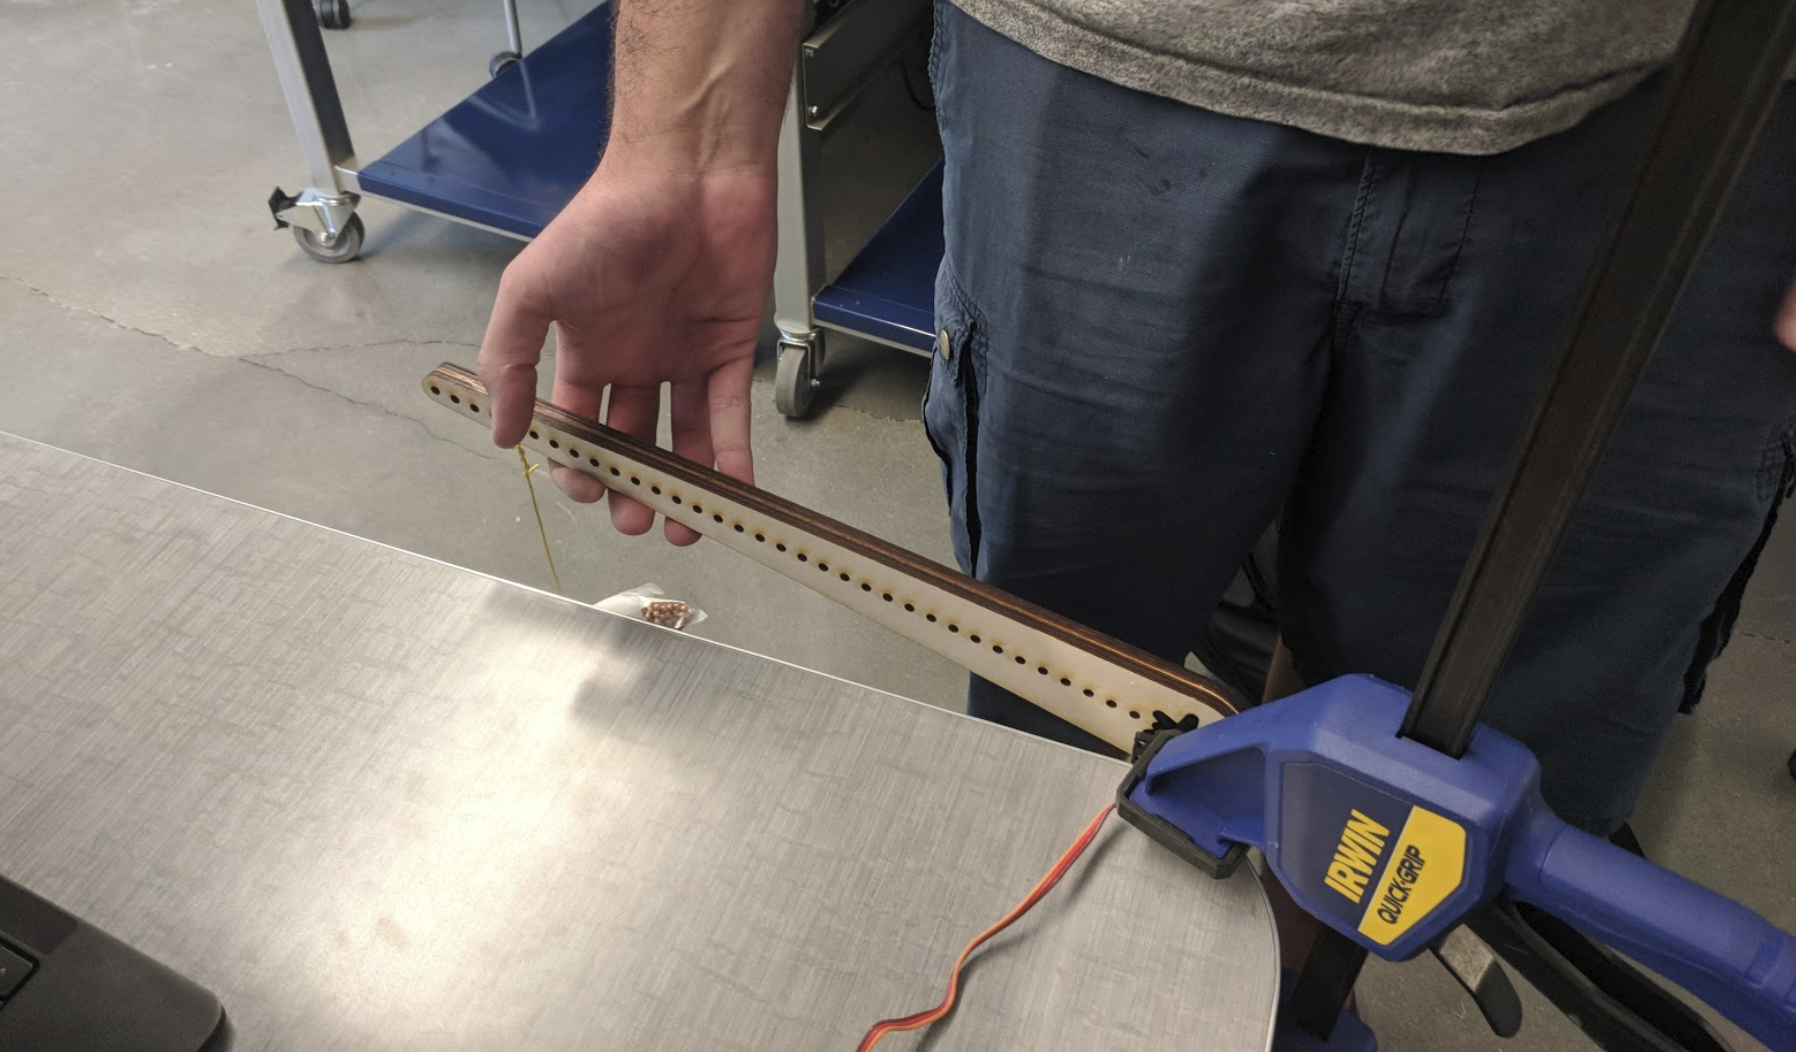
\includegraphics[width=0.7\textwidth]{figures/TestingMotors.png}
                    \caption{Testing the Jx-Servo HV-5932MG}
                    \label{fig:MotorTesting}
                \end{figure}        

        \subsubsection{Kinematics and Analysis}
        
            With any robot there is math and analysis that needs to be done to make sure that the robot will properly do what you want it to. The majority of the math that was done for Smallkat was to ensure we had a proper kinematic representation of the robot so that we could control the robot as well as analysis it. As mentioned before kinematics provide us with a mathematical way to describe the position of the robot in space. This can be done by describing the lengths and angles of each joint and figuring out where in space the robot is (forward kinematics) or by giving a point in space and figuring out was the angles needed to reach that point are (inverse kinematics). The forward kinematics were solved by using the D-H convention. The inverse kinematics were a little bit trickier and required a little more algebra. In order to solve this problem we had to apply everything we knew about inverse kinematics for a 3 degree of freedom leg and apply it to a 4 degree of freedom leg. With a redundant 4 dof system like ours, the leg has an additional limb inline with several others causing infinite solutions if you are just trying to solve the kinematics for an X,Y,Z point in space. As a result an additional term is added in to define the angle of the fourth link giving the system at most two solutions for a given x,y,z and theta value. Looking at the picture below you can see how this was done. By giving the leg an x,y,z value and an angle you can use some simple trigonometry to solve for an x,y,z the describes the 3 dof system which we already know how to solve for. 
            % add in pictures of 4 dof vs 3 dof kinematics
            % talk about jacobian and force propogation
            % try and get table or picture of results from torques
            % simulation a trajectory
            % center of mass calculations for final design in results
            % add calculations for tail kinematics - design was implemented after but needed research for how to control
        
        \subsubsection{Tail Design}
            When looking at other quadrupeds, tails are often not used, as they add complexity in the design. However, we saw a tail as an opportunity to better control our center of mass of the robot. This would give the user more body control, and could be removed if needed. We ultimately looked at two different designs for the tail: a solid tail and a continuum tail. A solid tail has articulation at the base of the tail, and is relatively simple to control. All normal kinematics and dynamics apply to model the movement of the tail, and modeling the system is relatively straight forward. Users can use a solid tail to move a mass left and right to control the center of mass of the robot as a whole.

            Continuum tails, on the other hand, are a series of linkages that are controlled by pulling on a string running through the linkages, similar to how fingers work in a hand. Motion is determined by how much actuators pull on the three or more strings built into the linkage. Modeling continuum tails is significantly more difficult, since every linkage has to be modeled as its own joint and link, complicating the system. However, users have some more control over the center of mass of the tail, especially if you stack continuum manipulators on top of one another.

            In order to give users an option, both a continuum tail and a solid tail were developed, and can be swapped out to simulate different situations. Figure \ref{fig:TailComparison} shows the difference between a solid and a continuum tail.
            
            \begin{figure}[H]
                \centering

                \caption{SmallKat's Solid Tail [Left] vs Continuum Tail [Right]}
                \label{fig:TailComparison}
            \end{figure}
        
        % add info and pictures regarding pla and ninja flex
        
        
        
            
        \subsubsection{Design Iterations} 
         
         % use pictures from google docs
         % add full prototype design
         % work up to final desing
         
         
         
         \paragraph{Sizing SmallKat}
            When deciding the size of SmallKat, we looked into the options currently provided on the market, as well as previous versions (talked about in Section \ref{subsec:SmallKatVersions}). Larger robots like Boston Dynamics' BigDog and Spot Mini robots were rather large, and would increase the cost of the robot as a whole. When looking at SmallKat V2, we appreciated its "desktop" size, but realized it's small form factor also limited us in our goals. Since deciding on an exact size was difficult, we decided to size our robot based on a standard servo. This would allow users to swap motors with others that better suit their needs without having to redesign the whole robot. In the end, our robot ended up being slightly larger than a standard house cat. While the robot is still small and relatively nimble, it also has the capability to have advanced sensors, like a 3D RealSense camera, and to traverse paths that the smaller SmallKats couldn't, like stairs. 

        \subsubsection{Head Design}
            Design decisions for the head were based on two different factors: look and ability to mount sensors. The look itself was taken from previous versions of SmallKats, and was scaled to for the size of the robot. The head is also designed to comfortably hold an Intel RealSense D400 series camera, to allow users to give SmallKat perception capability.

 
                
        
    
    % \subsection{Electronics}
    %     \subsubsection{Requirements}
    %         \begin{Deliverables}
    %             \item Custom boards for common interface:
    %             \subitem - Motor Controller built into motor
    %             \subitem - Continuum Tail Controller
    %             \subitem - Inertial Measurement Unit (IMU)
    %             \subitem - Foot Pressure Sensors
    %             \subitem - Motherboard
    %             \item Daisy Chain Communication Protocol
    %         \end{Deliverables}
        
    %     \subsubsection{Why Design Custom Boards?}

        % \subsubsection{Communication Protocol}


    \subsection{Electronics \& Low-Level Software}
        \subsubsection{Requirements}
            \begin{Deliverables} % im gonna make this a paragraph if i should even keep it here
                \item Low latency communication
                \item Feedback on position and torque from servo
                \item Minimal wires to manage
                \item Tunable PID constants
                \item Custom Foot Pressure Sensors
                \item High Speed Micro Controller
                \item Low latency, accurate IMU
            \end{Deliverables}

        \subsubsection{Motor Extra info}
        Each of these motors was researched and then the solution to make our own hybrid motor, using the body and motor and gearbox of the HV-5932MG and implementing a custom motor controller board. This was done to allow for position, velocity and torque control to be done directly on the Servo as well as to allow for tunable PID constants, and feedback to the master controller. This custom servo motor will communicate is a custom written daisy chained SPI protocol. These custom motor controllers will have a STM32 micro controller and an MA702 absolute magnetic encoder\cite{MA702}.
        \paragraph{Frequency}
        When designing the motor controllers 2 hardware timers were used for Pwm pins which would allow for up to \~4MHz pwm signals to be used. In the preliminary stages of testing an arbitrary value was chosen which equated to \~1MHz switching frequency. When testing the motor controllers an issue that occured, mainly while testing positional control. When given a set point the motor would only actuate given a duty cycle of  \~50\% this led us to testing a range of frequencies between 10kHz and 2Mhz. We found that a frequency of 20kHz allowed for a smooth motion of the motor without an un-pleasant sound.  
        \paragraph{Testing} 
        The custom motor controllers went through multiple stages of testing and development. starting with the designing of the preliminary version of the board. When doing this the pre-existing physical locations had to be taken into consideration, these include the center of the output shaft, the dimensions of the servo housing and the location of the motor itself. These locations would be the determining external dimensions of the board, the location of the MA702 absolute magnetic encoder and the mounting location being directly to the power connector of the motor. After populating and assembling this version of the board minor errors were discovered with a foot print and other minor details. These issues were fixed and the boards reordered. When the updated version was received, it was tested and independently the motors worked. When daisy chained the effect of SPI cross talk became eminent. The chaining of MISO and MOSI would result in the encoder input of a 0x00 or null byte to pull the output of the next motors encoder low and vice-versa. This problem was solved by using 2 dedicated SPI channels, one for communication between motors and the other to be used for intra-motor communication. 

        \subsubsection{Micro-Controllers}
            The project will require many micro controllers, each motor, foot sensor and IMU will require its own independent micro controller to communicate back to a master micro controller. Due to this two specific micro controllers were chosen, the STM32H743iit\cite{STM32H43IIT} and the STM32L432kb\cite{STM32l432KB}. The STM32H732iit was chosen for its large amount of flash memory at 1Mb, six dedicated hardware SPI channels, high clock speed of 400 MHZ being the fastest low cost micro controller easily available and its ability to emulate a usb HID device for low latency communication between the micro controller and a computer. The STM32L432kb was chosen due to its low cost and high clock speed of 80 Mhz. The STM32L432kb is used in each motor to perform 3 PID controllers and drive each motor, each foot sensor to collect all pressure sensor data ann report back to the master in order to remove the wait time between the reading of each sensor and each IMU to collect all the gyroscope and acceleration data and report it to the master controller in order to reduce the time taken to read the IMU. 
            
            
        \subsubsection{IMU}
            When deciding on the IMU to use for this project there was a lot of consideration taken to the specific model chosen, IMUs from STMicroelectronics, Bosch Sensortec and many other were considered but primarily the LSM303CTR, LSM6DS3USTR, BMX055, BMI160 and the BNO055\cite{BNO055} were considered. The BNO055 was chosen due to the great deal of available support available for the sensor, the on board fusing of the 3 major sensors on board and the previous experience the group has had with the sensor. The BNO055 fuses the gyroscope, magnetometer and accelerometer in order to stabilize the measurements being read.  
            
        \subsubsection{Foot Pressure Sensors}
        There was a large amount of existing research for these foot pressure sensors done by other groups. These include articles from Harvard\cite{chuah2012composite}\cite{chuah2014enabling}, WPI\cite{youssefian2014contact} and MIT\cite{tenzer2014inexpensive}. The research done by the group for the paper "Inexpensive and Easily Customized Tactile Array Sensors using MEMS Barometers Chips" \cite{chuah2012composite} proved to be the most relevant when it cam to understanding the affect the encapsulation of the sensors would have. Due to their documentation using the MPL115A2 pressure sensor we were able to get a baseline for the optimal thickness of polyurethane to use for our project. We used the BMP280 barometric pressure sensor \cite{BMP280} as it had a much higher working range as well as greater sensitivity. The BMP280 pressure sensor allowed for a 24 bit pressure reading, the availability to use SPI to communicate with the sensor making it far easier to communicate with multiple sensors made it a simple choice.
        \begin{figure}[H]
            \centering
            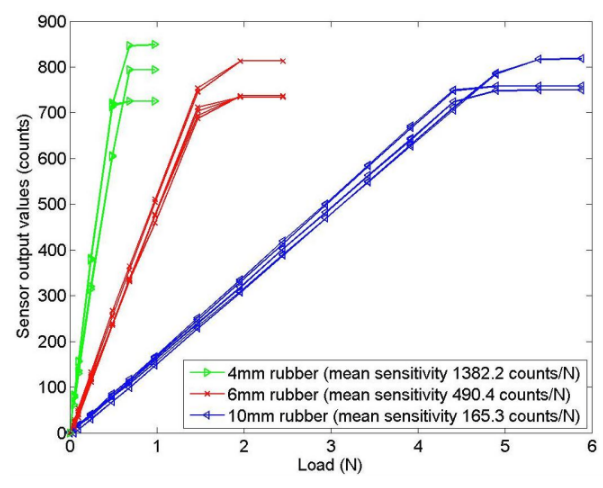
\includegraphics[width=0.5\textwidth]{figures/Load_vs_SensorvsThickness.png}
            \caption{Correlation between load and pressure readings at different thicknesses of polyurethane\cite{chuah2012composite}}
            \label{fig:ThicknessVSPressure}
        \end{figure}

        The research done by the Contact Behavior of Soft Spherical Tactile Sensors\cite{youssefian2014contact} group demonstrated a similar method for calculating a pressure vector using magnets and hall effect sensors, despite the difference the math used to convert from readings to a pressure vector proved very useful to calculate out pressure vector using the 7 sensors on the foot of the robot. 
        \subsubsection{Communication Protocol}
            \paragraph{Processor cycles}
                The main purpose of the motherboard is to receive data from the computer over USB HID, parse, process and distribute to the motors accordingly. After speaking with Boston dynamics and deciding that for a reliable dynamics controller we would ideally have a control loop speed of \~ 1kHz at the highest level. This means that in 1 ms the micro controller must receive 64 bytes of data from the on board computer, parse it to determine the type of command being sent to the motors, whether it is a position, velocity or torque set point, populate the buffer and send through SPI to each motor assuming all read and writes to memory and GPIO is atomic, the time for data transfer can be calculated. \newline
                \begin{figure}[!t]
                \begin{minipage}{0.5\textwidth}
                    \begin{gather*}
                        \text{Clock Speed} = 384 \text{MHz}\\
                        \text{Data Size} = 16 \text{bits}\\
                        \text{SPI Transfer Speed} = 24 \tiny{\frac{\text{Mbits}}{\text{s}}}\\
                        \text{Size of SPI Package}= 5\\
                        \text{ No. Devices} = 5\\
                        \\
                        \\
                        \textbf{Time per clock cycle}\\
                        \frac{1}{\text{Clock Speed}}\\
                        \frac{1}{384000000}\\
                        = 2.5*10^{-9}\text{s}\\
                        \\
                        \\
                        \textbf{No. bits per leg}\\
                        \text{Data Size} * \text{Size of SPI Package} * \text{No. Devices}\\
                        = 16 \tiny{\frac{\text{bits}}{\tiny{\text{packet}}}} * 5\frac{\text{packets}}{\text{device}} * 5\text{Devices} \\
                        = 400 \tiny{\frac{\text{bits}}{\text{leg}}}\\
                        \\
                        \\
                    \end{gather*} 
                \end{minipage}
                \begin{minipage}{0.5\textwidth}
                    \begin{gather*} 
                        \textbf{No. Clock cycles per SPI bit}\\
                        \frac{\text{Clock Speed}}{\text{SPI	Transfer Speed}}\\
                        \tiny{\frac{384\text{MHz}}{24\frac{\text{MHz}}{\text{s}}}}\\ 
                        =16\tiny{\text{Clock Cycles}}\\
                        \\
                        \\
                        \textbf{Time to update a single leg}\\
                        \text{No. Clock cycles per SPI bit} * \text{Time per clock cycle}\\
                        16 * 2.5*10^{-9}\\
                        =4*10^{-8}\text{s}\\
                        \\
                        \\
                        \textbf{Time to update all legs}\\
                        \text{Time to update a single leg} * \text{No. Legs}\\
                        4*10^{-8}* 4\\
                        =1.6*10^{-7}\text{s}\\
                    \end{gather*}  
                \end{minipage}
                \caption{Calculations to determine number of clock cycles elapsed during SPI transmission}
                \label{fig:SPIClockCycles}
                \end{figure}

                Using the same SPI channel and DMA, the total time to transfer all data to each of the legs would be \~ 1.6*10$^{-7}$s, this will allow the USB packet to be received, transmitted to the motors and the updated data returned to to the computer via an updated USB packet. \newline
            
            Continuing with the assumption of atomic data transfers the use of separate SPI channels for each leg would allow for update speeds of 4*10$^{-8}$s minimizing the total time in between receiving and sending a return packet. This would be the optimal solution as it allows us to keep the 1ms round trip for usb to be keot as well as allowing for other processes to be run.  
            
            \paragraph{Micro-controller to Micro-controller}
            The decision on how to communicate between the master micro controller and the multiple salves through out the system came down to ease of re usability. The major communication options included ${I^2c}$, SPI, Can Bus, RS485 serial and RS232 Serial. The following is a table giving pros and cons of each choice.
        \begin{table}[H]
            \centering
            \begin{tabular}{|p{2cm}|p{6cm}|p{6cm}|}
        \hline
        Protocol   & Pros & Cons \\
        \hline
            \multirow{4}{*}{${I^2c}$} & Simple 2 wire interface & Requires independent addresses on each device \\
            & Easy Daisy chaining & Requires independent firmware to be flashed to each motor \\
            & Available on most micro controllers & Non synchronous \\
            & Supports DMA & Requires motor to be re flashed to move to a different location \\
            \hline
            \multirow{6}{*}{SPI} & Synchronous & Requires 4 wires to interface \\
            & Max baud rate of ~16.5 Mbaud &   \\
            & Supports DMA &  \\
            & Available on most microcontrollers & \\
            & Daisychainable & \\
            & Allows for multiple slaves to share one chip select line therefore no addressing & \\
            \hline
            \multirow{2}{*}{Can Bus} & Designed to be daisy chained  & Not available on most micro controllers \\
            & Simple 2 Wire interface & Slow  \\
            \hline
            \multirow{3}{*}{RS485 Serial}& Simple to use & Requires external IC\\
            &Designed to daisy chain & Slow \\
            & & Requires a software address be set\\
            \hline
            \multirow{3}{*}{RS232 Serial}& Available on most micro controllers & Slow\\
            & Simple to use & non synchronous \\
            & No hardware addresses needed & Difficult to daisy chain but possible\\
            
        \hline
        \end{tabular}
            \caption{Pros \& Cons of each communication protocol}
            \label{tab:ProsConsCommunicationProtocols}
        \end{table}
        After researching in depth into each of these protocols taking into development time, limitation of resources such as space on circuit boards and ease of communication between micro controllers chosen, SPI was the final choice. The micro controllers used in the servo, foot pressure sensor and IMU breakout boards communicate back to the master micro controller through a daisy chained SPI DMA protocol where the packet of data is sent to the first object in the chain, the reply from the previous cycle is passed on as a return packet to the next, and so on until the final packet reaches the final micro controller and returns the packet of results to the main micro controller. The flow of data for an example leg is shown in the figure below.
        \begin{figure}[H]
        \centering
        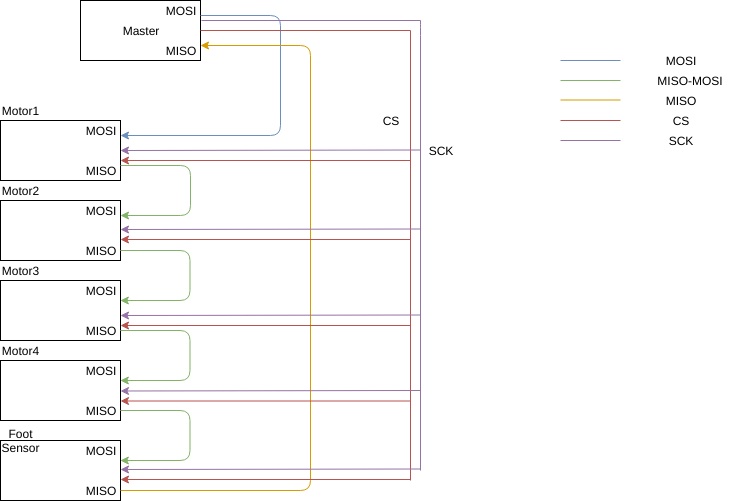
\includegraphics[width=0.6\textwidth]{figures/Leg_Flow_Dragram.png}
        \caption{Flow of data through a leg}
        \label{fig:DataFlow_Leg}
        \end{figure}
            \paragraph{Micro-controller to Computer}
            There were many fewer options for communicating between a computer and the master micro controller. The major solutions included Ethernet, USB HID and uart over USB. These options each have their advantages and disadvantages. Ethernet, this requires external supporting circuitry to interface between the micro controller and computer, this combined with the priority level of the networking stack on any Debian distribution of Linux including Ubuntu eliminated this option as a viable solution. Usart over USB was a viable option as the USB communication stack is marginally higher than the networking stack however usb to Usart is limited to \~2 Mbits/s. This meant that the throughput would not be enough for the robot to function reliably. USB HID communicates a 54 kbyte packet, reliably at 1ms. The HID USB stack is also the communication stack with the highest priority in any Debian based Linux system. therefore it is the least likely to lose a packet or have a data transmission error. 

    
    \subsection{High Level Software: Robot Kernel}
        The kernel's main job will be to run the kinematics and dynamics engine. This includes balancing, foot-step planning, and all gaits to be developed (see gait section). To speed up development time and decrease cycle-times in certain calculations, an existing platform should ideally be used. The ideal platform has the following criteria:
        \begin{enumerate}
            \item Real-time performance with a guaranteed cycle time of under 1ms 90\% of the time (not including communication time with the Motherboard)
            \item Able to be interface with the communication protocols to be used
            \item Open-source and easily to work with
            \item Programming language agnostic (preferred)
        \end{enumerate}

        \paragraph*{The Final Decision: Bowler Kernel}
        Bowler Kernel is a low level platform designed to run at high speeds on linux machines. The entire system is also developed in Java. Bowler Kernel along with Bowler Studio was used on the previous SmallKats (V2 and V2.1). Bowler Kernel is extremely powerful when used correctly. It has a built-in kinematics engine and a default walking gait designed for general use. It creates a 'virtual robot' in an .xml document, which contains the dimensions of the real robot. Bowler Kernel also allows for more compartmentalized code than other systems, since parameters like DH Conventions, don't have to be manually inputed into the code. However, it also makes the whole system slower at run-time. Bowler Kernel is also very complex, since it attempts to have a lot of different features with little to no documentation.

        In the end, we decided to go with Bowler Kernel due to its inter-process communication (IPC) tools and our access to its creator, Kevin Harrington. One of our many goals was to develop a simple user interface. Since Bowler Kernel has a UDP Socket tool, we were able to send data, like joint angles and speeds, to a computer wirelessly, with minimal development overhead. You can read more about this in our Results Section. Additionally, having access to Kevin Harrington, the creator of Bowler Kernel and Bowler Studio, allows for us to get around the lack of documentation.

        \paragraph*{IHMC Open Robotics Software}
        The IHMC Open Robotics Software is a library set developed by Florida Institute for Human and Machine Cognition (IHMC) designed to make it easier to develop bipedal and quadrupedal walking platforms. It includes a physics simulator and a kinematics calculator written in Java that will allow speedy calculations with close to real-time performance, while still offering a simple and robust development platform. The IHMC library can be split into two parts: the kinematics engine and the simulator.

        The kinematics engine built into the IHMC library uses the Euclid Core library (also developed by IHMC) to calculate matrices and perform rigid body transformations. Since this library is designed in Java, the main concern is its performance in a real-time environment. However, if designed properly, Java code can actually be faster on subsequent runs than a C++ or C application can be. This is because the Java Runtime Environment (also known as the Java Virtual Machine, or JVM) can optimize certain parts of the code by making assumptions after the first instance has run. This is true as long as the developer is careful to avoid using the garbage collector built into the JVM, since it is very computationally intensive. Java also makes development easier, since Gradle can be used to manage and pull together libraries when compiling into an executable. Finally, Java applications are cross-platform, so one executable can be run on any device with a JVM. This makes deployment on several different robots easy, since executables can be compiled locally before pushed to other robots running different processors.

        The IHMC libraries also include a simulator designed to prototype software. It allows to simulates any developed code at its core instead of risking hardware. The simulator is also better integrated with the other libraries to be used, since it is developed by the same group.

        \paragraph*{Robot Operating System (ROS)}
        ROS, or Robot Operating System, is a widely used open-source robotics platform designed for adaptability and ease-of-bring-up for new robotic platforms. There are currently two major versions of ROS: ROS 1 and ROS 2.

        ROS 1 has been tried and tested in the real world for over a decade. It is written in C and C++ and uses TCP/IP to communicate between processes, or nodes. ROS 1 is a really powerful tool for research and development, due to its adaptability and customizability. ROS's biggest advantage is the shear amount of packages developed for it. From camera software to SLAM algorithms to kinematics engines, ROS 1's community adoption along its open-source nature has led to a surplus of open-source packages that makes development easier. However, ROS 1 has two major downfalls: its speed and its security. Since ROS 1 is built using a networking back-end, the communication speeds between nodes is slow and unreliable. Testing proved that the guaranteed real-time performance for ROS 1 is about 100ms, about 100x slower than what we need for our system. It also relies on all ports to be open for good communication, making it a security nightmare. Most robotic solutions are initially developed in ROS for quick development time, but are then ported to a custom platform once key algorithms and functions are developed. Other research and development platforms, similar to ours, use ROS as a user interface and testing suite, with custom software written to communicate with ROS and the hardware.

        ROS 2 is an attempt to fix the multitude of problems with ROS 1. It uses UDP sockets instead of the TCP/IP protocol for faster communication between nodes. It also implements new security protocols as a part of the platform. It is also built in a way where any language can be used, because its core is easily wrapped by any modern language. 
        However, ROS 2 still has its issues. For starters, ROS 2 is relatively new: just a few years old in a semi-stable form. It is not very feature-rich, and is not backwards compatible with ROS 1 packages (there is a backwards compatibility tool, but is very buggy at the time of writing). The second big problem is the instability of speed. ROS 2 boasts that it has been built to be real-time. However testing this claim, we found that although it could guarantee a 1ms loop 95\% of the time, the cycle time varied greatly - from 10 microseconds to 2.7 milliseconds. Although ROS 2 may be very viable in this situation, we determined it's relatively young life as well as its low adoption in the industry made it impracticable for use.

        \paragraph*{Custom Platform}
        Since neither ROS nor Bowler Studio is exactly what we were looking for, a custom platform could have been written. It would be likely written in C and C++ and communicate through processes using a standard inter-process communication protocol, or IPC. This would allow for our platform to be extremely fast, limited only by the Linux kernel and processor speed, while maintaining all communication open locally. It can also be easily adapted to send data over other protocols, like SPI, USB, or TCP/IP or UDP Sockets. However, developing a custom platform is a project in itself, and adds a lot of development time and work to ensure proper stability and functionality. As fun as it sounded, we determined it was outside the scope of our project.

        \subsubsection{User Control System}
        The user control system will have several functions. Its first and for-most job is to act as a human-to-robot interface (HRI). This includes visualizing the current physical state of the robot as well as allowing a user the capability to control the robot. The user control system will also act as a debugging system for the developer. The ideal platform for this use-case meets the following criteria

        \begin{enumerate}
            \item 3D robot visualizer that displays the current physical state of the robot
            \item Able to send commands to the kernel to control the robot
            \item Easy to set up cross computer communication
            \item Able to display any relevant error messages to the user.
            \item Open-source and easily modifiable
            \item Preferably capable of interfacing with other complex sensors like cameras and LIDAR systems for future development
        \end{enumerate}

        \paragraph*{The Final Decision: Custom User Interface over UDP}


        \paragraph*{ROS Kinetic}
        The Robot Operating System (ROS) excels in the world of human-to-robot interaction and interfacing with complex sensors. It's lack of maintainable speed is not a big factor, since a user interface that updates once every 100 milliseconds is still a very usable and functional interface. ROS also allows easy expansion of SmallKat's capabilities in the future: adding an Intel RealSense camera with ROS's many perception packages allow for a robust SLAM implementation. ROS also contains many visualization packages to help the user debug the robot.

        % \subsubsection{High-Level Controller}
        % In the end, we decided to use Bowler Studio for the High-Level Controller. It offers cross-platformability and easy development due to its Java backbone. It also is relatively stable although not used much in the industry.

        % \subsubsection{Localization and User Control Software}
        % For the Localization and User Control Software, we decided on using ROS 1 due to its stability and wide range of open-source packages. The Localization and User Control Software will be split into two major sections: Visualization and Mapping, and User Control.

        % \paragraph*{Visualization and Mapping}
        % Visualization and Mapping will be utilizing the multitude of SLAM and navigation algorithms built into ROS 1. It takes in input from the on-board camera, and provides direction and velocity to the High-Level Controller. This allows us to easily implement a fully autonomous robot capable of exploring new areas.

        % \paragraph*{User Control}
        % The user control feature will have two parts: control and supervision. The control part will allow users to initiate gaits and control them remotely from another computer. It will also allow for initiating the autonomy function built in to SmallKat. The supervision portion will give the user the capability of watching different key variables, like joint angles, relative position, and body position relative to the world. This will help with debugging while developing on SmallKat.
        
        \subsubsection{Controls Equations}
        \begin{table}[H]
            \centering
            \begin{tabular}{|c|c|c|c|c|}
            \hline
                Link & d & $\theta$ & r & $\alpha$\\
                \hline
                1 & 0 & $\theta_1$ & 0 & 90 \\
                2 & 0 &$\theta_2$ & $l_1$ & 0  \\
                3 & 0 &$\theta_3$ & $l_2$ & 0 \\
                4 & 0 &$\theta_4$ & $l_3$ & 0  \\
                \hline
                \end{tabular}
            \caption{Table of DH parameters}
            \label{tab:DHTable}
        \end{table}
        
        \begin{figure}[H]
        \centering
        \begin{gather*}
        X = a_3*sin(\theta_2+\theta_3)+a_2*sin(\theta2)+a_4*sin(\theta_2+\theta_3+\theta_4)\\
        Y = sin(\theta_1)*(a_1+a_3*cos(\theta_2+\theta_3)+a_2*cos(\theta_2)+a_4*cos(\theta_2+\theta_3+\theta_4))\\
        Z = -cos(\theta_1)*(a_1+a_3*cos(\theta_2+\theta_3)+a_2*cos(\theta_2)+a_4*cos(\theta_2+\theta_3+\theta_4))
        \end{gather*}
        
        \caption{Forward Positional Kinematics}
        \label{fig:FWKin_Robot}
        \end{figure}
        
        % \begin{figure}[H]
        % \centering

        % \[
        % J=
        %   \begin{bmatrix}
        %   0& a_3*c(\theta_{2+3})+a_2*c(\theta_{2+3+4})& a_3*c(\theta_{2+3})+a_4*c(\theta_{2+3+4})& a_4*c(\theta_{2+3+4})\\
        %   c(\theta_1)*(a_1 + a_3*c(\theta_{2+3}) + a_2*c(\theta_2) + a_4*c(\theta_{2+3+4}))&-s(1)*(a_3*s(\theta_{2+3}) + a_2*s(\theta_2) + a_4*s(\theta_{2+3+4}))&-s(\theta_1)*(a_3*s(\theta_{2+3}) + a_4*s(\theta_{2+3+4}))&-a_4*s(\theta_{2+3+4})*s(\theta_1)
        %   \end{bmatrix}
        
        % \]
        

        % \caption{Forward torque Kinematics}
        % \label{fig:FW_TorqueKin}
        % \end{figure}

        %end

%% This Should go in the Implementation section
Based on our research we have decided to take make advancements in what is considered the typical quadrupedal design. We intend on creating a system that more closely resembles a cat by implementing 4 DOF legs and a continuum tail. Our electronic systems will include pressure sensing feet with multiple sensors to allow for the triangulation of the pressure vectors, an adaptive number of IMUs which can be placed in optimal locations and custom smart servo motors capable of performing constant position, velocity and torque. We will be creating custom control systems that will allow us to implement a variety of gaits. We hope to be able to at least create a basic walking and running gait and experiment with jumping.


\subsection{Low-Level Control Software} 
    The low level control software of the robot can be broken down into four distinct subcategories. These include the master controller, foot sensors, motors and IMUs. 
        \subsubsection{Master Controller}
        This controller receives trajectory points from the computer over USB HID, the controller then parses the data received to each motor. This controller performs calculations in order to optimize leg trajectory and paths. The data is packaged into four byte packets shown below.  
        \begin{figure}[H]
        \centering
        \begin{tabular}{|c|c|c|c|c|}
        \hline
        Device ID& Command & Val 1 & Val 2 & Val 3\\
        \hline
        \end{tabular}
        \caption{Data packet structure}
        \label{fig:DataPacketStructure}
        \end{figure}
        The data is then sent to the motors, foot sensors and any other devices connected in the chain. Due to the nature of the system the data must be sent in order of the last device first as shown below. 
        \begin{figure}[H]
        \centering
        \begin{tabular}{|c|c|c|c|c|}
        \hline
            Foot Sensor & Motor 4 & Motor 3 & Motor 2 & Motor 1  \\
            \hline
        \end{tabular}
        \caption{Order of packets sent to a leg}
        \label{fig:PacketOrder}
        \end{figure}
        The path of data follows the structure below.

        \begin{longtable}{|r|p{0.9\textwidth}|}
        \hline
        Packet & Action of data\\
        \hline
        {Packet 1} &  {\begin{itemize}
                        \item Motor 1 Receives the Foot Sensor packet, replies previous position, velocity and torque to motor 2
                        \item Motor 2 Receives return data from Motor 1 and replies its data to Motor 3
                        \item Motor 3 Receives return data from Motor 2 and replies its data to Motor 4 
                        \item Motor 4 Receives return data from Motor 3 and replies its data to the foot sensor 
                        \item The foot Sensor Receives return data from Motor 4 and replies the readings from the pressure sensors to the master controller
                    \end{itemize}}\\
                    \hline
        {Packet 2} &  {\begin{itemize}
                        \item Motor 1 Receives the Motor 4 packet, replies the Foot Sensor packet to motor 2
                        \item Motor 2 Receives the Foot Sensor packet and replies Motor 1 data to Motor 3
                        \item Motor 3 Receives return data from Motor 1 and replies Motor 2 data to Motor 4 
                        \item Motor 4 Receives return data from Motor 2 and replies Motor 3 data to the foot sensor 
                        \item The foot Sensor Receives return data from Motor 3 and replies Motor 4 data to the master controller
                    \end{itemize}}\\
                    \hline
        {Packet 3} &  {\begin{itemize}
                        \item Motor 1 Receives the Motor 3 packet, replies the Motor 4 packet to motor 2
                        \item Motor 2 Receives the Motor 4 packet and replies the Foot Sensor packet to Motor 3
                        \item Motor 3 Receives the Foot Sensor packet and replies Motor 1 data to Motor 4 
                        \item Motor 4 Receives return data from Motor 1 and replies Motor 2 data to the foot sensor 
                        \item The foot Sensor Receives return data from Motor 2 and replies Motor 3 data to the master controller
                    \end{itemize}}\\
                    \hline
        {Packet 4} &  {\begin{itemize}
                        \item Motor 1 Receives the Motor 2 packet, replies the Motor 3 packet to motor 2
                        \item Motor 2 Receives the Motor 3 packet and replies the Motor 4 packet to Motor 3
                        \item Motor 3 Receives the Motor 4 packet and replies Motor 1 data to Motor 4 
                        \item Motor 4 Receives the Foot Sensor packet and replies Motor 1 data to the foot sensor 
                        \item The foot Sensor Receives return data from Motor 1 and replies Motor 2 data to the master controller
                    \end{itemize}}\\
                    \hline
        {Packet 5} &  {\begin{itemize}
                        \item Motor 1 Receives the Motor 1 packet, replies the Motor 2 packet to motor 2
                        \item Motor 2 Receives the Motor 2 packet and replies the Motor 3 packet to Motor 3
                        \item Motor 3 Receives the Motor 3 packet and replies Motor 4 packet to Motor 4 
                        \item Motor 4 Receives the Foot Sensor packet and replies Motor 1 data to the foot sensor 
                        \item The foot Sensor receives Foot Sensor packet and replies Motor 1 data to the master controller
                    \end{itemize}}\\
        \hline
        \end{longtable}

        \noindent Once the cycle is completed the motors update the PID controllers, the foot sensors collect the pressure data and the cycle is looped. The return packet order is shown below.
        \begin{figure}[H]
        \centering
        \begin{tabular}{|c|c|c|c|c|}
        \hline
            Motor 1 & Motor 2 & Motor 3 & Motor 4 & Foot Sensor \\
            \hline
        \end{tabular} 
        \caption{Order of Data returned from a leg}
        \label{fig:DataReturnOrder}
        \end{figure}

        \subsubsection{Motor Controllers}
            When the motor receives a packet it checks if the first byte if the packet and compares it to the Dev ID of the motor. If the device Id does not match the first byte of the packet it is stages for transmission on the next packet received. If the packet is used to update that motor, the second byte of the packet is checked and compared to different known options. 
            \begin{table}[H]
                \centering
                \begin{tabular}{|c|c|}
                \hline
                    Value & Command \\
                    \hline
                    0x22 & Update device ID based on byte 3 of the packet\\
                    0x47 & Updates Position PID constants based on bytes 3,4,5 of the packet \\
                    0x48 & Updates Velocity PID constants based on bytes 3,4,5 of the packet \\
                    0x49 & Updates Torque PID constants based on bytes 3,4,5 of the packet \\
                    0x91 & Updated position setpoint in Postion PID loop\\
                    0x92 & Updated position setpoint in Velocity PID loop\\
                    0x93 & Updated position setpoint in Torque PID loop\\
                    \hline
                    \end{tabular}
                \caption{Command values for servo}
                \label{tab:ServoCommandValues}
            \end{table}
            In between receiving packets the motors run multiple PID loops simultaneously to control position, torque and velocity at an ~161kHz refresh rate.
        \subsubsection{IMU}
            The IMU micro controller continuously samples the BNO055, recording the current gyroscope, acceleration and magnetometer data. On request from the master controller the IMU checks byte 1 and compares it to the device ID, if it matches it compares byte 2 to the list of known commands and replies accordingly which can be see below.
            \begin{table}[H]
                \centering
                \begin{tabular}{|c|c|}
                \hline
                    Value & Command \\
                    \hline
                    0x22 & Update device ID based on byte 3 of the packet\\
                    0x37 & get gyroscope data\\
                    0x38 & get accelerometer data\\
                    0x39 & get magnetometer data\\
                    \hline
                    \end{tabular}
                \caption{Command values for IMU}
                \label{tab:IMUCommandValues}
            \end{table}

        \subsubsection{Foot Sensor}
            Smurlarly to the IMU, the foot sensor micro controller continuously samples the 7 pressure sensors. On request from the master controller the foot sensor checks byte 1 and compares it to the device ID, if it matches it compares byte 2 to the list of known commands and replies accordingly which can be see below.
            \begin{table}[H]
                \centering
                \begin{tabular}{|c|c|}
                \hline
                    Value & Command \\
                    \hline
                    0x22 & Update device ID based on byte 3 of the packet\\
                    0x32 & return most recent foot pressure sensor readings\\
                    \hline
                    \end{tabular}
                \caption{Command values for Foot sensor}
                \label{tab:FootSensorCommandValues}
            \end{table}
